% Name: Matrix with its size marked
% Description: An m by n matrix with braces naming its rows and columns, and one entry, row i and column j, picked out.
% Tags: matrix, dimensions, braces, linear algebra

\usetikzlibrary{decorations.pathreplacing, fit, matrix}

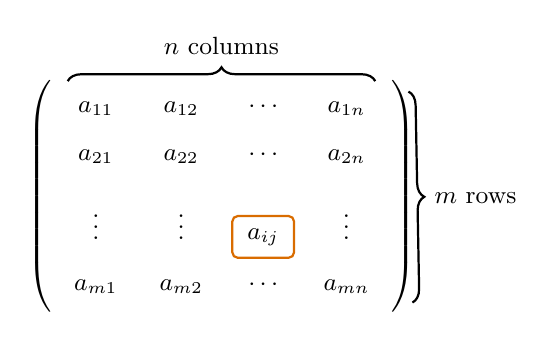
\begin{tikzpicture}[every node/.style={font=\small}]
  \matrix (A) [matrix of math nodes, left delimiter={(}, right delimiter={)}, row sep=2mm, column sep=3mm, nodes={minimum width=7mm}] {
    a_{11} & a_{12} & \cdots & a_{1n} \\
    a_{21} & a_{22} & \cdots & a_{2n} \\
    \vdots & \vdots & a_{ij} & \vdots \\
    a_{m1} & a_{m2} & \cdots & a_{mn} \\
  };
  \node[draw, orange!85!black, thick, rounded corners=2pt, fit=(A-3-3), inner sep=1pt] {};
  \draw[decorate, decoration={brace, amplitude=5pt, raise=4pt}, thick] (A-1-1.north west) -- node[above=10pt] {$n$ columns} (A-1-4.north east);
  \draw[decorate, decoration={brace, amplitude=5pt, raise=12pt}, thick] (A-1-4.north east) -- node[right=17pt] {$m$ rows} (A-4-4.south east);
\end{tikzpicture}
